\documentclass{article}

\usepackage{amsmath, amsthm, amssymb, amsfonts}
\usepackage{thmtools}

% ------------------------------------------------------------------------------
\usepackage{graphicx}
\graphicspath{ {./images/} }
% ------------------------------------------------------------------------------

\usepackage{setspace}
\usepackage{geometry}
\usepackage{float}
\usepackage{hyperref}
\usepackage[english]{babel}
\usepackage{framed}
\usepackage[dvipsnames]{xcolor}
\usepackage{tcolorbox}
\usepackage{minted}

% ------------------------------------------------------------------------------
% \usepackage{times}
% \usepackage{fontspec}
% \setmainfont{Ubuntu Nerd Font}
% \setsansfont{Noto Sans}
% \setmonofont{FiraCode Nerd Font}
% ------------------------------------------------------------------------------

\colorlet{LightGray}{White!90!Periwinkle}
\colorlet{LightOrange}{Orange!15}
\colorlet{LightGreen}{Green!15}

\newcommand{\HRule}[1]{\rule{\linewidth}{#1}}

\declaretheoremstyle[name=Theorem,]{thmsty}
\declaretheorem[style=thmsty,numberwithin=section]{theorem}
\tcolorboxenvironment{theorem}{colback=LightGray}

\declaretheoremstyle[name=Proposition,]{prosty}
\declaretheorem[style=prosty,numberlike=theorem]{proposition}
\tcolorboxenvironment{proposition}{colback=LightOrange}

\declaretheoremstyle[name=Principle,]{prcpsty}
\declaretheorem[style=prcpsty,numberlike=theorem]{principle}
\tcolorboxenvironment{principle}{colback=LightGreen}

\setstretch{1.2}
\geometry{
    textheight=9in,
    textwidth=5.5in,
    top=1in,
    headheight=12pt,
    headsep=25pt,
    footskip=30pt
}

% ------------------------------------------------------------------------------

\begin{document}

% ------------------------------------------------------------------------------
% Cover Page and ToC
% ------------------------------------------------------------------------------

\title{ \normalsize \textsc{}
\\ [2.0cm]
\HRule{1.5pt} \\
\LARGE \textbf{\uppercase{Data Communications and
	Networking}
\HRule{2.0pt} \\ [0.6cm] \LARGE{Chapter 09} \vspace*{10\baselineskip}}
}
\date{}
\author{\textbf{Rising Flare Community} \\
	Made with ArchLinux and vscode (\LaTeX workshop).
}

\maketitle
\begin{center}
	Source code is available on \href{https://github.com/SharafatKarim/pstu-cse-academic/blob/main/semester%203/cce/networking%20exercises/ch%208/cce_ch8.tex}{GitHub}. 
	Feel free to do changes or improvements. Use xetex to compile the tex file instead of using \LaTeX directly for avoiding font issues.
\end{center}
\newpage

\tableofcontents
\newpage

% ------------------------------------------------------------------------------

\section{Questions}
\subsection{
	Distinguish between communication at the network layer and communication
	at the data-link layer.
}

The network layer is responsible for routing packets from the source to the destination. It is responsible for logical addressing and routing.

The data-link layer is responsible for transferring data between two devices on the same network. It is responsible for physical addressing and error detection.

\subsection{
	Distinguish between a point-to-point link and a broadcast link.
}

A point-to-point link is a link between two devices. It is used to transfer data between two devices.

A broadcast link is a link between multiple devices. It is used to transfer data between multiple devices.

\subsection{
	Can two hosts in two different networks have the same link-layer address?
	Explain.
}

Yes, two hosts in two different networks can have the same link-layer address. The link-layer address is used to identify the device on the same network. The link-layer address is unique on the same network, but it can be the same on different networks.

\subsection{
	Is the size of the ARP packet fixed? Explain.
}

No, the size of the ARP packet is not fixed. The size of the ARP packet depends on the type of hardware and protocol used.

\subsection{
	What is the size of an ARP packet when the protocol is IPv4 and the hardware
	is Ethernet?
}

Typically the size of ARP packet is 28 bytes. Here's a breakdown,

\begin{enumerate}
	\item Hardware type: 2 bytes
	\item Protocol type: 2 bytes
	\item Hardware address length: 1 byte
	\item Protocol address length: 1 byte
	\item Operation: 2 bytes
	\item Sender hardware address: 6 bytes
	\item Sender protocol address: 4 bytes
	\item Target hardware address: 6 bytes
	\item Target protocol address: 4 bytes
\end{enumerate}

\subsection{
	Assume we have an isolated link (not connected to any other link) such as a
	private network in a company. Do we still need addresses in both the network
	layer and the data-link layer? Explain.
}

No, we do not need addresses in both the network layer and the data-link layer. If the link is isolated, we only need addresses in the data-link layer to identify the devices on the same network.

\subsection{
	In Figure 9.9, why is the destination hardware address all 0s in the ARP
	request message?
}

\begin{figure}[H]
	\center
	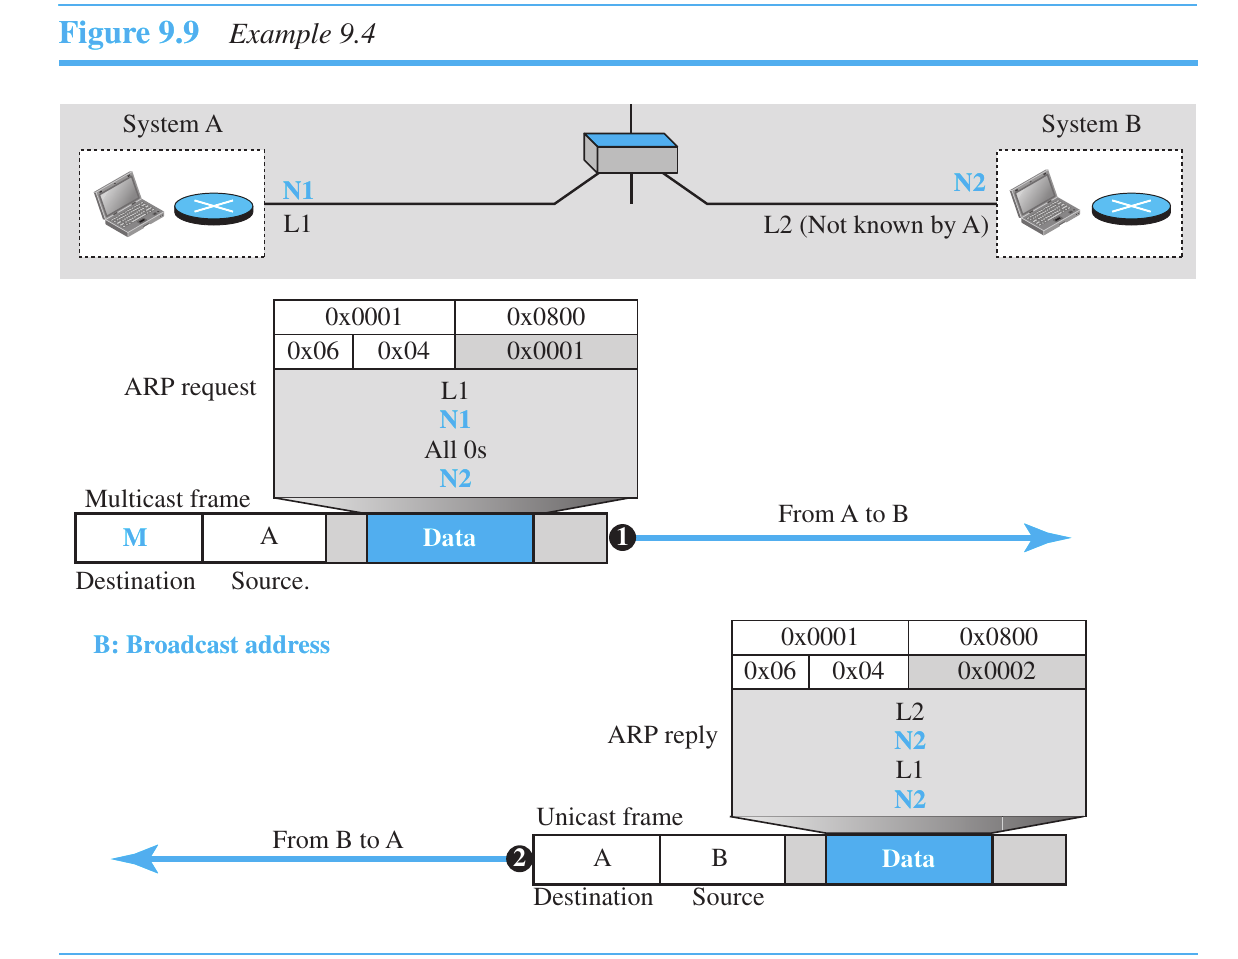
\includegraphics[scale=0.5]{9.9.png}
	\caption{9.9}
\end{figure}

The destination hardware address is all 0s in the ARP request message because the destination hardware address is not known.

\subsection{
	In Figure 9.9, why is the destination hardware address of the frame from A to
	B a broadcast address?
}

The destination hardware address of the frame from A to B is a broadcast address because the destination hardware address is not known. The frame is broadcast to all devices on the same network.

\subsection{
	In Figure 9.9, how does system A know what the link-layer address of system
	B is when it receives the ARP reply?
}

System A sends an ARP request to all devices on the same network. System B receives the ARP request and sends an ARP reply to system A. From the ARP reply, system A knows the link-layer address of system B. In the reply message, the link-layer address of system B is included.

When system A receives the ARP reply, it updates its ARP cache with the link-layer address of system B. The ARP cache is used to store the link-layer address of the devices on the same network.

\subsection{
	When we talkabout the broadcast address in a link, do we mean sending a
	message to all hosts and routers in the link or to all hosts and routers in the
	Internet? In other words, does a broadcast address have a local jurisdiction or
	a universal jurisdiction? Explain.
}

When we talk about the broadcast address in a link, we mean sending a message to all hosts and routers on the same network.

The broadcast address has a local jurisdiction. It is used to send a message to all devices on the same network.

\subsection{
	Why does a host or a router need to run the ARP program all of the time in the
	background?
}

The ARP program is used to resolve the IP address to the link-layer address. The ARP program is run all the time in the background to update the ARP cache with the link-layer address of the devices on the same network.

\subsection{
	Why does a router normally have more than one interface?
}

A router normally has more than one interface to connect to multiple networks. Each interface is used to connect to a different network. The router uses the interfaces to route packets between the networks.

\subsection{
	Why is it better not to change an end-to-end address from the source to the
	destination?
}

It is better not to change an end-to-end address from the source to the destination because the address is used to identify the source and destination devices. If the address is changed, the packets will not reach the destination.

\subsection{
	How many IP addresses and how many link-layer addresses should a router
	have when it is connected to five links?
}

A router connected to five links should have five IP addresses and five link-layer addresses. Each link has a different IP address and link-layer address.

% ------------------------------------------------------------------------------
% ------------------------------------------------------------------------------
% ------------------------------------------------------------------------------

\section{Problems}
\subsection{
	Assume we have an internet (a private small internet) in which all hosts are
	connected in a mesh topology. Do we need routers in this internet? Explain.
}

No, we do not need routers in this internet. In a mesh topology, all hosts are connected to each other. The packets can be routed from the source to the destination without the need for routers.

\subsection{
	In the previous problem, do we need both network and data-link layers?
}

No, we do not need both network and data-link layers. In a mesh topology, the hosts are connected to each other. The data can be transferred between the hosts without the need for network layer.

Also for security reasons, we can use both network and data-link.

\subsection{
	Explain why we do not need the router in Figure 9.15.
}
\begin{figure}[H]
	\center
	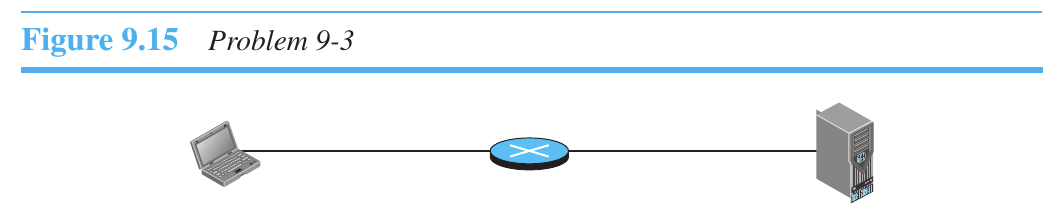
\includegraphics[scale=0.5]{9.15.png}
	\caption{9.15}
\end{figure}

As we can see in the figure, the hosts are connected to each other. So, the packets can be routed from the source to the destination without the need for a router.

\subsection{
	Explain why we may need a router in Figure 9.16.
}
\begin{figure}[H]
	\center
	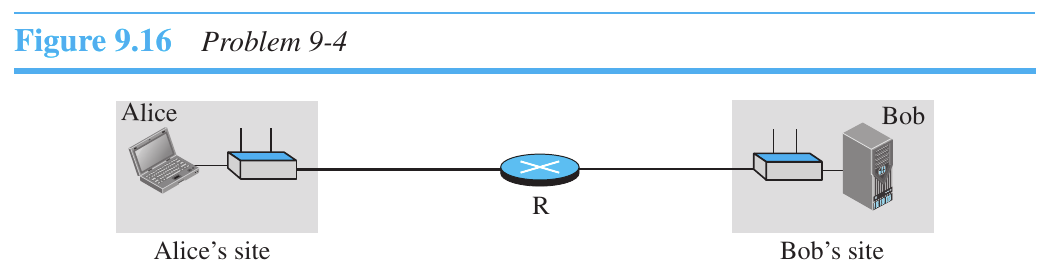
\includegraphics[scale=0.5]{9.16.png}
	\caption{9.16}
\end{figure}

As we can see in the figure, the hosts are in difference networks. Here, Alice and Bob are in their own individual network.
That's why the packets cannot be routed from the source to the destination without the need for a router.

\subsection{
	Is the current Internet using circuit-switching or packet-switching at the data-link layer? Explain.
}

The current Internet uses packet-switching at the data-link layer because it is more efficient and flexible than circuit-switching. Packet-switching does not require a dedicated communication channel to be established before data can be transmitted, and it allows data to be sent over different paths.

\subsection{
	Assume Alice is travelling from 2020 Main Street in Los Angeles to 1432 American
	Boulevard in Chicago. If she is travelling by air from Los Angeles Airport to
	Chicago Airport,
}
% a. find the end-to-end addresses in this scenario.
% b. find the link-layer addresses in this scenario.
\begin{enumerate}
	\item \textbf{ Find the end-to-end addresses in this scenario. }
	      \begin{itemize}
		      \item Source address: 2020 Main Street, Los Angeles
		      \item Destination address: 1432 American Boulevard, Chicago
	      \end{itemize}
	\item \textbf{ Find the link-layer addresses in this scenario. }
	      \begin{itemize}
		      \item Source address: Los Angeles Airport
		      \item Destination address: Chicago Airport
	      \end{itemize}
\end{enumerate}

\subsection{
	In the previous problem, assume Alice cannot find a direct flight from the Los
	Angeles to the Chicago. If she needs to change flights in Denver,
}
% a. find the end-to-end addresses in this scenario.
% b. find the link-layer addresses in this scenario.
\begin{enumerate}
	\item \textbf{ Find the end-to-end addresses in this scenario. }
	      \begin{itemize}
		      \item Source address: 2020 Main Street, Los Angeles
		      \item Destination address: 1432 American Boulevard, Chicago
	      \end{itemize}
	\item \textbf{ Find the link-layer addresses in this scenario. }
	      \begin{itemize}
		      \item Source address: Los Angeles Airport
		      \item Middle address: Denver Airport
		      \item Final destination address: Chicago Airport
	      \end{itemize}
\end{enumerate}

\subsection{
	When we send a letter using the services provided by the post office, do we
	use an end-to-end address? Does the post office necessarily use an end-to-end
	address to deliver the mail? Explain.
}

Yes, we use an end-to-end address when we send a letter using the services provided by the post office. The post office not necessarily uses the end-to-end address to deliver the mail to the destination.

\subsection{
	In Figure 9.5, assume Link 2 is broken. How can Alice communicate with
	Bob?
}
\begin{figure}[H]
	\center
	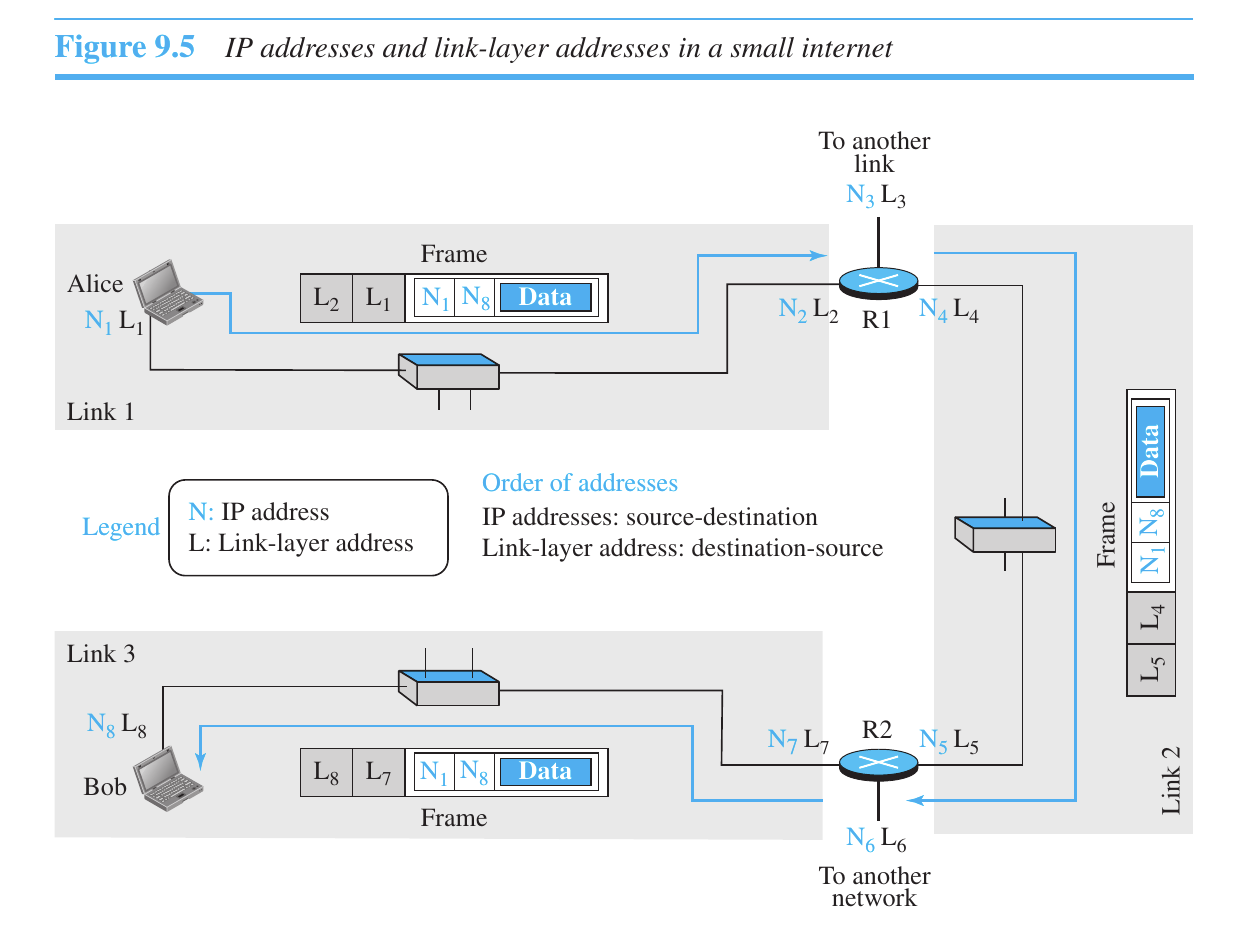
\includegraphics[scale=0.5]{9.5.png}
	\caption{9.5}
\end{figure}
In Figure 9.5, if Link 2 is broken, Alice has to communicate with Bob through a different path.

\subsection{
	In Figure 9.5, show the process of frame change in routers R1 and R2.
}
The process of frame change in routers R1 and R2 is as follows:
\begin{itemize}
	\item R1 receives the frame from Alice and changes the link-layer address to the link-layer address of R2.
	\item R1 sends the frame to R2.
	\item R2 receives the frame from R1 and changes the link-layer address to the link-layer address of Bob.
	\item R2 sends the frame to Bob.
\end{itemize}

In the internet in Figure 9.5, we have three links and two routers. We also have
shown only two hosts: Alice (source) and Bob (destination). For each host, we have
shown two addresses, the IP addresses (N) and the link-layer addresses (L). Note
that a router has as many pairs of addresses as the number of links the router is con-
nected to. We have shown three frames, one in each link. Each frame carries the
same datagram with the same source and destination addresses (N1 and N8), but the
link-layer addresses of the frame change from link to link. In link 1, the link-layer
addresses are L 1 and L 2. In link 2, they are L 4 and L 5. In link 3, they are L7 and L8 .
Note that the IP addresses and the link-layer addresses are not in the same order. For
IP addresses, the source address comes before the destination address; for link-layer
addresses, the destination address comes before the source. The datagrams and frames are designed in this way, and we follow the design. \\

\textbf{Check the image and text-book for more details. Above texts are directly copied from the text-book.}

\subsection{
	In Figure 9.7, assume system B is not running the ARP program. What would
	happen?
}
\begin{figure}[H]
	\center
	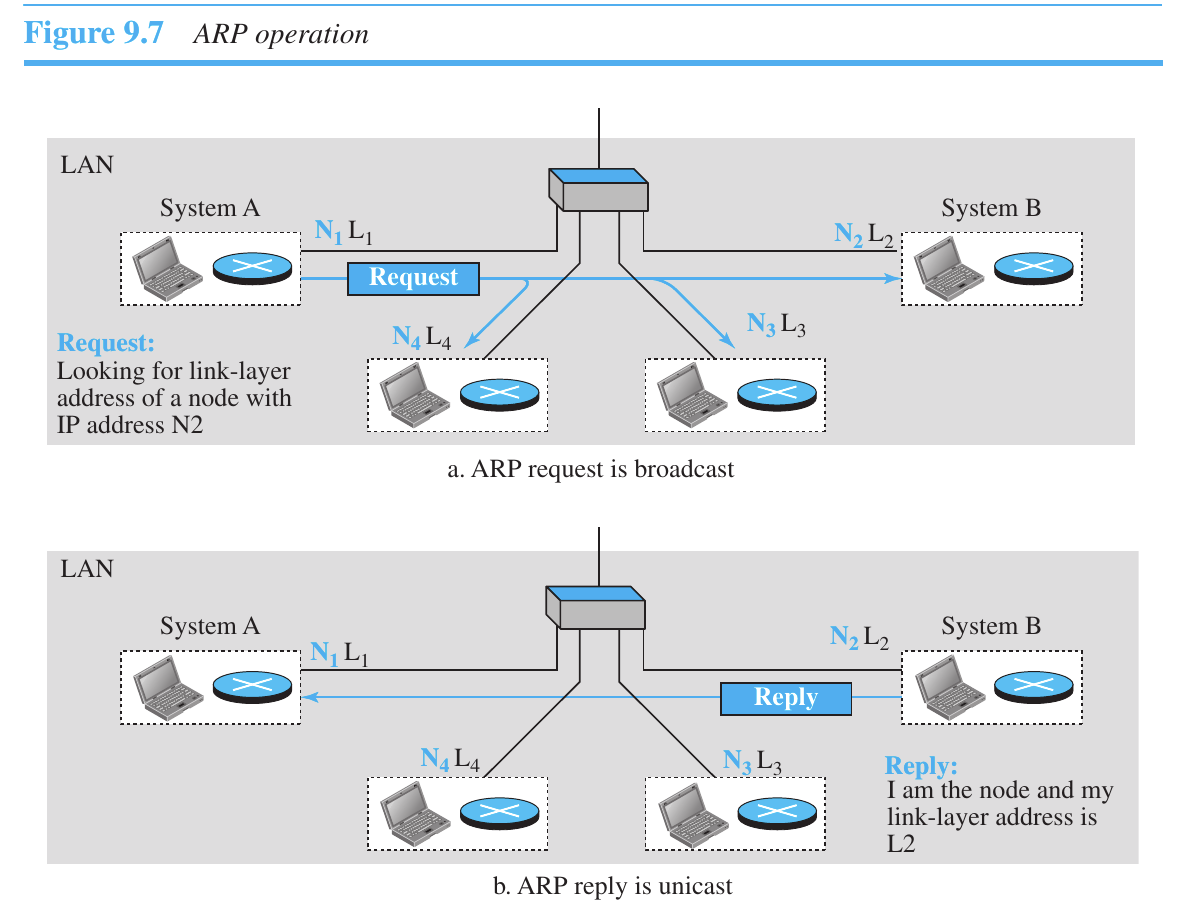
\includegraphics[scale=0.5]{9.7.png}
	\caption{9.7}
	\label{fig:9.7}
\end{figure}

In Figure 9.7, if system B is not running the ARP program, system A cannot send the ARP request to system B. The ARP request is used to resolve the IP address to the link-layer address. If system B is not running the ARP program, system A cannot resolve the IP address to the link-layer address of system B.

\subsection{
	In Figure 9.7, do you think that system A should first check its cache for mapping from N2 to L2 before even broadcasting the ARP request?
	Assume the network in Figure 9.7 does not support broadcasting. What do you
	suggest for sending the ARP request in this network?
}

In Figure 9.7, system A should first check its cache for mapping from N2 to L2 before broadcasting the ARP request. If the mapping is found in the cache, system A can send the frame directly to system B without the need for ARP request.

If the network in Figure 9.7 does not support broadcasting, system A can send the ARP request to the router. The router can forward the ARP request to system B. System B can send the ARP reply to the router, and the router can forward the ARP reply to system A.

\subsection{
	In Figures 9.11 to 9.13, both the forwarding table and ARP are doing a kind of
	mapping. Show the difference between them by listing the input and output of
	mapping for a forwarding table and ARP.
}

The difference between the forwarding table and ARP is as follows:

\textbf{For figure 9.11:}
\begin{itemize}
	\item \textbf{ Forwarding table: }
	      \begin{itemize}
		      \item Input: \( N_B \)
		      \item Output: \( N_1 \)
	      \end{itemize}
	\item \textbf{ ARP: }
	      \begin{itemize}
		      \item Input: \(N_1\)
		      \item Output: \(L_1\)
	      \end{itemize}
\end{itemize}

\textbf{For figure 9.12:}
\begin{itemize}
	\item \textbf{ Forwarding table: }
	      \begin{itemize}
		      \item Input: \( N_B \)
		      \item Output: \( N_3 \)
	      \end{itemize}
	\item \textbf{ ARP: }
	      \begin{itemize}
		      \item Input: \(N_3\)
		      \item Output: \(L_3\)
	      \end{itemize}
\end{itemize}

\textbf{For figure 9.13:}
\begin{itemize}
	\item \textbf{ Forwarding table: }
	      \begin{itemize}
		      \item Input: \( N_B \)
		      \item Output: \( N_B \)
	      \end{itemize}
	\item \textbf{ ARP: }
	      \begin{itemize}
		      \item Input: \(N_B\)
		      \item Output: \(L_B\)
	      \end{itemize}
\end{itemize}

\textbf{Please use text-book for images. You can directly deduce above parameteres from image.}

\subsection{
	Figure 9.7 shows a system as either a host or a router. What would be the
	actual entity (host or router) of system A and B in each of the following cases:
}
% a. If the link is the first one in the path?
% b. If the link is the middle one in the path?
% c. If the link is the last one in the path?
% d. If there is only one link in the path (local communication)?

\begin{enumerate}
	\item \textbf{ If the link is the first one in the path? }
	      \begin{itemize}
		      \item System A: Host
		      \item System B: Router
	      \end{itemize}
	\item \textbf{ If the link is the middle one in the path? }
	      \begin{itemize}
		      \item System A: Router
		      \item System B: Router
	      \end{itemize}
	\item \textbf{ If the link is the last one in the path? }
	      \begin{itemize}
		      \item System A: Router
		      \item System B: Host
	      \end{itemize}
	\item \textbf{ If there is only one link in the path (local communication)? }
	      \begin{itemize}
		      \item System A: Host
		      \item System B: Host
	      \end{itemize}
\end{enumerate}

Figure \ref{fig:9.7} (9.7) is provided at page \pageref{fig:9.7}


\vspace{10cm}
\textbf{
	Life is a series of decisions, you never have unlimited options or unlimited time to think, but what you choose in that instant defines who you are. 
}
\begin{flushright}
	-Kyojuro Rengoku
\end{flushright}

\end{document}
